\documentclass[german]{latex4ei/latex4ei_sheet}

\title{Example\\ Cheat Sheet}
\author{Konstantin Späth}					% optional, delete if unchanged
\myemail{duell10111@t-online.de}	

\begin{document}

\section{Grundbegriffe Wahrscheinlichkeit}

\begin{sectionbox}
	\subsection{Mengen- und Boolsche Algebra}
	\begin{tablebox}{lll}
		%& $(P(\Omega);\capdot , \cupplus, \overline{A};\Omega,\emptyset )$\\ \mrule
		Kommutativ 		& $A \capdot B = B \capdot A$ & $A \cupplus B = B \cupplus A$\\
		Assoziativ 		& \multicolumn{2}{l}{ $(A \capdot B) \capdot C = A \capdot (B \capdot C)$} \\
		& \multicolumn{2}{l}{$(A \cupplus B) \cupplus C = A \cupplus (B \cupplus C)$} \\
		Distributiv 	& \multicolumn{2}{l}{$A \capdot (B \cupplus C) = (A \capdot B) \cupplus (A \capdot C)$}\\
		& \multicolumn{2}{l}{ $A \cupplus (B \capdot C) = (A \cupplus B) \capdot (A \cupplus C)$}\\ \cmrule
		Indempotenz		& $A \capdot A = A$ & $A \cupplus A = A$\\
		Absorbtion		& $A \capdot (A \cupplus B) = A$ & $A \cupplus (A \capdot B) = A$\\
		Neutralität		& $A \capdot \Omega = A$ & $A \cupplus \emptyset = A$\\
		Dominant		& $A \capdot \emptyset = \emptyset$ & $A \cupplus \Omega = \Omega$\\
		Komplement		& $A \capdot \overline{A} = \emptyset$ & $A \cupplus \overline{A} = \Omega$\\
		& $\overline{\overline{A}} = A$ & $\ol{\Omega} = \emptyset$\\
		De Morgan		& $\overline{A \capdot B} = \overline{A} \cupplus \overline{B}$ & $\overline{A \cupplus B} = \overline{A} \capdot \overline{B}$\\
	\end{tablebox}
\end{sectionbox}
	
\begin{sectionbox}
	\subsection{Kombinatorik}
	Mögliche Variationen/Kombinationen um $k$ Elemente von maximal $n$ Elementen zu wählen bzw. $k$ Elemente auf $n$ Felder zu verteilen:
	\begin{tablebox}{l|cc}
		& \large Mit Reihenfolge & \large Reihenfolge egal\\ \cmrule
		%& ungleiche Elemente & gleiche Elemente \\
		\large Mit Wiederholung & \large $n^k$ & \Large $\binom{n+k-1}{k}$\\[0.2em]
		\large Ohne Wiederholung & \Large $\frac{n!}{(n-k)!}$ & \Large $\binom nk$\\
	\end{tablebox}
	Permutation von $n$ mit jeweils $k$ gleichen Elementen: $\frac{n!}{k_1 ! \cdot k_2 ! \cdot ...}$ \\
	$\binom nk = \binom n{n-k} = \frac{n!}{k! \cdot (n-k)!}$ \quad $\binom 42 = 6$ \quad $\binom 52 = 10$
\end{sectionbox}

\begin{sectionbox}
	\subsection{Grundbegriffe}

	\begin{tablebox}{ll}
		Tupel & $(i,j) \neq (j,i)$ für $i \neq j$ \\
		Ungeordnetes Paar & $\{i,j\} = \{j,i\}$ \\
		Potenzmenge & $\mathbb \P(\Omega)$ ist Menge aller Teilmengen von $\Omega$ \\
	\end{tablebox}
\end{sectionbox}

\begin{sectionbox}
	\subsection{Integralarten}

	\renewcommand{\arraystretch}{1.6}
	\begin{tablebox}{ccc}
		$F(x)$ & $f(x)$ & $f'(x)$ \\ \cmrule
		$\frac{1}{q+1}x^{q+1}$ & $x^q$ & $qx^{q-1}$ \\
		\raisebox{-0.2em}{$\frac{2\sqrt{ax^3}}{3}$} & $\sqrt{ax}$ & \raisebox{0.2em}{$\frac{a}{2\sqrt{ax}}$}\\
		$x\ln(ax) -x$ & $\ln(ax)$ & $\textstyle \frac{1}{x}$\\
		%e^x & e^x & e^x \\
		$\frac{1}{a^2} e^{ax}(ax- 1)$ & $x \cdot e^{ax}$ & $e^{ax}(ax+1)$ \\
		$\frac{a^x}{\ln(a)}$ & $a^x$ & $a^x \ln(a)$ \\
	\end{tablebox}
	\vspace{-8pt}
	\begin{tablebox}{ll}
		$\int \frac{\diff t}{\sqrt{at+b}} = \frac{2 \sqrt{at+b}}{a}$ & $\int t^2 e^{at} \diff t = \frac{(ax-1)^2+1}{a^3} e^{at}$\\
		$\int t e^{at} \diff t = \frac{at-1}{a^2} e^{at}$ & $\int x e^{ax^2} \diff x = \frac{1}{2a} e^{ax^2}$\\
	\end{tablebox}
\end{sectionbox}

\begin{sectionbox}
	\subsection{Binome, Trinome}
	$(a\pm b)^2 = a^2 \pm 2ab + b^2$ \hfill $a^2 - b^2 = (a-b)(a+b)$\\
	$(a \pm b)^3 = a^3 \pm 3a^2b + 3ab^2 \pm b^3$\\
	$(a+b+c)^2 = a^2 + b^2 + c^2 + 2ab + 2ac + 2bc$
\end{sectionbox}

% SECTION ====================================================================================
\section{Bedingte Wahrscheinlichkeit und \newline Unabhängigkeit}
% ============================================================================================
%Wechselseite Information $I(A,B) = \log_2 \frac{\P_B (A)}{\P(A)}$\\ % Wichtig für Aufgaben?
%Es gilt: $\P(A \cap B) = \P(A) - \P(A \cap B^\complement)$\\
\begin{sectionbox}
	\subsection{Bedingte Wahrscheinlichkeit}
	Bedingte Wahrscheinlichkeit für $A$ falls $B$ bereits eingetreten ist:\\
	$\P_B(A) = \P(A|B) = \frac{\P(A \cap B)}{\P(B)}$\\ %\qquad\quad $\P(B|A) = \P(A|B) \frac{\P(B)}{\P(A)}$\\

	\subsubsection{Totale Wahrscheinlichkeit und Satz von Bayes}
	Es muss gelten: $\bigcup\limits_{i \in I} B_i = \Omega$ für $B_i \cap B_j = \emptyset$, $\forall i \neq j$ \\
	\begin{tabular}{ll}
		Totale Wahrscheinlichkeit: & $\P(A) = \sum\limits_{i \in I} \P(A|B_i)\P(B_i)$\\
		Satz von Bayes: & $\P(B_k | A) = \frac{\P(A | B_k)\P(B_k)}{\sum\limits_{i \in I} \P(A|B_i) \P(B_i)}$\\
	\end{tabular}


	\subsubsection{Multiplikationssatz}
	$\P(A \cap B) = \P(A|B)\P(B) = \P(B|A)\P(A)$
	\\ \\
	Beliebig viele Ereignisse:\\
	$\P\left(A_1 \cap A_2 \cap \shdots \cap A_k\right) \newline
	= \P\left(A_{\pi(1)}\right)\P\left(A_{\pi(2)}|A_{\pi(1)}\right)\P\left(A_{\pi(3)}|A_{\pi(2)} \cap A_{\pi(1)}\right) \times \newline
	\shdots \times \P\left(A_{\pi(k)}|A_{\pi(k-1)} \cap \shdots \cap A_{\pi(1)}\right)$
\end{sectionbox}

\begin{sectionbox}
	\subsection{Stochastische Unabhängigkeit}
	Ereignise $A$ und $B$ sind unabhängig falls:\\
	$\P(A \cap B) = \P(A)\P(B)$ \\
	$\Rightarrow \P(B|A)=\P(B)$  \\ \\
	\textbf{Allgemein:}  \\
	$\P\left(\bigcap\limits_{i \in J} A_i\right) = \prod\limits_{i \in J}\P\left(A_i\right)$
	mit Indexmenge $I$ und $\emptyset \neq J \subseteq I$
\end{sectionbox}

\section{Zufallsvariablen}
% ============================================================================================
\begin{sectionbox}
	\subsection{Definition}
	$\X : \Omega \mapsto \Omega'$ ist Zufallsvariable, wenn für jedes Ereignis $A' \in \F'$  \\
	im Bildraum ein Ereignis $A$ im Urbildraum $\F$ existiert, \\
	sodass $\left\{\omega \in \Omega|\X(\omega) \in A'\right\} \in \F$\\ \\
\end{sectionbox}

\begin{sectionbox}
	\subsection{Unabhängigkeit von Zufallsvariablen}
	Zufallsvariablen $\X_1,\shdots,\X_n$ sind stochastisch unabhängig, wenn für jedes $\vec{x} = [x_1,\shdots,x_n]^\top \in \R^n$ gilt:
	\[\boxed{\P(\{\X_1 \leq x_1,\shdots,\X_n \leq x_n\}) = \prod\limits_{i=1}^{n}{\P(\{\X_i \leq x_i\})}}\]
	\underline{Gleichbedeutend:}\\
	\begin{tabular}{l}
		$F_{\X_1,\shdots,\X_n}(x_1,\shdots,x_n) = \prod\limits_{i=1}^{n}{F_{\X_i}(x_i)}$\\
		$p_{\X_1,\shdots,\X_n}(x_1,\shdots,x_n) = \prod\limits_{i=1}^{n}{p_{\X_i}(x_i)}$\\
		$f_{\X_1,\shdots,\X_n}(x_1,\shdots,x_n) = \prod\limits_{i=1}^{n}{f_{\X_i}(x_i)}$\\
	\end{tabular}
\end{sectionbox}

%Wechselseitige Information $I(x_i,y_j) = \log_2 \frac{p_{\X|\Y}(x_i|x_j)}{p_{\X}(x)}$\\
%Transinformation $I(\X,\Y)$\\
%Entropie und Transinforation
\begin{sectionbox}
	\subsection{Bedingte Zufallsvariablen}
	Bedingte Wahrscheinlichkeit für Zufallsvariablen:\\
	\begin{tabular}{ll}
		Ereignis A gegeben: & $F_{\X|A}(x|A) = \P\left(\eset{\X \le x} | A\right)$\\
		ZV $\Y$ gegeben: & $F_{\X|\Y}(x|y)= \P\left(\eset{\X \le x} | \eset{\Y = y}\right)$\\
		& $p_{\X|\Y}(x|y) = \frac{p_{\X,\Y}(x,y)}{p_{\Y}(y)}$\\
		& $f_{\X|\Y}(x|y) = \frac{f_{\X,\Y}(x,y)}{f_{\Y}(y)} = \frac{\diff F_{X|Y}(x|y)}{\diff x}$\\
	\end{tabular}

\end{sectionbox}

\section{Kontinuierlich Wahrscheinlichkeitsräume}


\begin{sectionbox}
    \subsection{Allgemeines}
    
    \begin{tablebox}{cc}
    
    Verteilfkt & 
    
    \end{tablebox}
        
    
\end{sectionbox}

\subsection{Kolomogorov-Axiome und $\sigma$-Algebren}

\begin{sectionbox}
    
    \subsubsection{$\sigma$-Algebren}
    Sei $\Omega$ eine Menge. Eine Menge A $\subseteq \mathcal{P}(\Omega)$ heißt $\sigma$-Algebra über $\Omega$, wenn folgende Eigenschaften erfüllt sind:
    
    \begin{enumerate}
        \item $\Omega \in A$
        \item Wenn $B \in A$, dann folgt $\overline{B} \in A$
        \item Für $n \in \N$ sei $C_{n} \in A$. Dann gilt auch $\bigcup_{n=1}^{\infty} C_{n} \in A$
    \end{enumerate}
    
    
\end{sectionbox}

\begin{sectionbox}
	\subsection{Wahrscheinlichkeitsmaß $\P$}
	$\P(A) = \frac{|A|}{|\Omega|}$ \hfill $\P(A \cup B) = \P(A) + \P(B) - \P(A \cap B)$\\
	\subsubsection{Axiome von Kolmogorow}
	\begin{tabular}{ll}
		Nichtnegativität: & $\P(A) \geq 0 \Ra \P:\mathbb F \mapsto [0,1]$ \\
		Normiertheit: & $\P(\Omega) = 1$ \\
		Additivität: & $\P\left(\bigcup\limits_{i=1}^{\infty} A_i \right) = \sum\limits_{i=1}^{\infty} \P(A_i)$, \\
		& wenn $A_i \cap A_j = \emptyset$, $\forall i \neq j$ \\
	\end{tabular}
	\subsubsection{Weitere Eigenschaften}
	\begin{itemize}
		\item 	$\P(\overline{A}) = 1 - \P(A)$
		\item 	$\P(\emptyset) = 0$ \qquad $\P(\Omega)=1$
		\item 	$\P(A \backslash B) = \P(A \cap \overline{B}) = \P(A) - \P(A \cap B)$
		\item 	$\P(A \cup B) = \P(A) + \P (B) - \P(A \cap B)$
		\item 	$\P(A \cap B) = \P(A) + \P (B) - \P(A \cup B)$
		\item 	$A \subset B \Rightarrow \P(A) \leq \P(B)$
		\item 	$\P(\bigcup_{i=1}^k A_i) \leq \sum_{i=1}^k \P(A_i)$
	\end{itemize}


\end{sectionbox}

% --------------------------------
% |Stochastische Standardmodelle |
% ~~~~~~~~~~~~~~~~~~~~~~~~~~~~~~~~
% SECTION ====================================================================================
\section{Stochastische Standardmodelle}
% ============================================================================================
\begin{sectionbox}
	\subsection{Begriffe}
	\textbf{Gedächtnislos}\\
	Eine Zufallsvariable X ist gedächtnislos, falls: \\
	$\P(\{\X > a + b)\} | \{\X > a\}) = \P(\{\X > b\})$, \qquad $a,b > 0$

\end{sectionbox}
\begin{sectionbox}
	\subsection{Gleichverteilung}
	\subsubsection{Diskret}
	$p_{\X}(x) = \frac{1}{|\Omega|}, \quad x \in \left\{1,\dots,\abs{\Omega}\right\}$\\
	\emph{Beispiele:} Wurf einer fairen Münze, Lottozahlen

	\subsubsection{Stetig ($a,b: -\infty < a < b < \infty$)}
	$f_{\X}(x) = \begin{cases}
	\frac{1}{b - a} & x \in [a,b] \\
	0 & \text{sonst} \\
	\end{cases}$
	\qquad
	$F_{\X}(x) = \begin{cases}
	0 & x < a \\
	\frac{x-a}{b - a} & x \in [a,b] \\
	1 & x > b \\
	\end{cases}$
	\\ \\  \\
	\everymath{\displaystyle}
	\begin{tablebox}{lll}
		$\underset{\text{Erwartungswert}}{\E[\X] =\frac{a+b}{2}}\quad\ $ & $\underset{\text{Varianz}}{\Var[\X] =\frac{(b-a)^2}{12}}$ & $\underset{\text{Charakt. Funktion}}{\varphi_{\X}(\cx s) = \frac{e^{j \omega b}-e^{j \omega a}}{j \omega (b-a)}}$\\
	\end{tablebox}
	\emph{Beispiele:} Winkel beim Flaschendrehen, Phase einer empf. Sinusschwingung

\end{sectionbox}
% ====================================================================================
\begin{sectionbox}
	\subsection{Bernoulliverteilung ($p \in [0,1]$)}
	\textbf{Wahrscheinlichkeitsmasse} \\
	2 Ereignisse: Erfolg und Misserfolg\\
	$p$: Wahrscheinlichkeit  \\ \\
	$p_{\X}(k) = \begin{cases}
	p, & k = 1 \\
	1-p & k = 0 \\
	0 & \text{sonst}\\
	\end{cases}$ \qquad\quad
	$F_{\X}(k) = \begin{cases}
	0, & k < 0 \\
	1-p & 0 \le k < 1 \\
	1 & k \ge 1\\
	\end{cases}$
	\\ \\  \\
	\everymath{\displaystyle}
	\begin{tablebox}{lll}
		$\underset{\text{Erwartungswert}}{\E[\X] = p}\quad\ $ & $\underset{\text{Varianz}}{\Var[\X] = p (1-p)}$ & $\underset{\text{Wahrscheinlichkeitserz. Funktion}}{G_{\X} (z) = pz + 1 -p}$
	\end{tablebox}
	\emph{Beispiele:} Einmaliger Wurf einer (unfairen) Münze
\end{sectionbox}

% ====================================================================================
\begin{sectionbox}
	\subsection{Binomialverteilung $\mathcal B(n,p)$ ($p \in [0,1], n \in \N$)}
	Folge von $n$ Bernoulli-Experimenten\\
	$p$: Wahrscheinlichkeit für Erfolg \\
	$k$: Anzahl der Erfolge \\
	\textbf{Wahrscheinlichkeitsmasse}
	\\
	$p_{\X}(k) = B_{n,p}(k) = \begin{cases}
	\binom{n}{k} p^k (1 - p)^{n - k} & k \in \left\{0,\dots,n\right\} \\
	0 & \text{sonst} \\
	\end{cases}$\\
	mit $\binom{n}{k} = \frac{n!}{k!(n-k)!}$
	\\
	\everymath{\displaystyle}
	\parbox{3.3cm}{\emph{WMF/PMF:} \\ 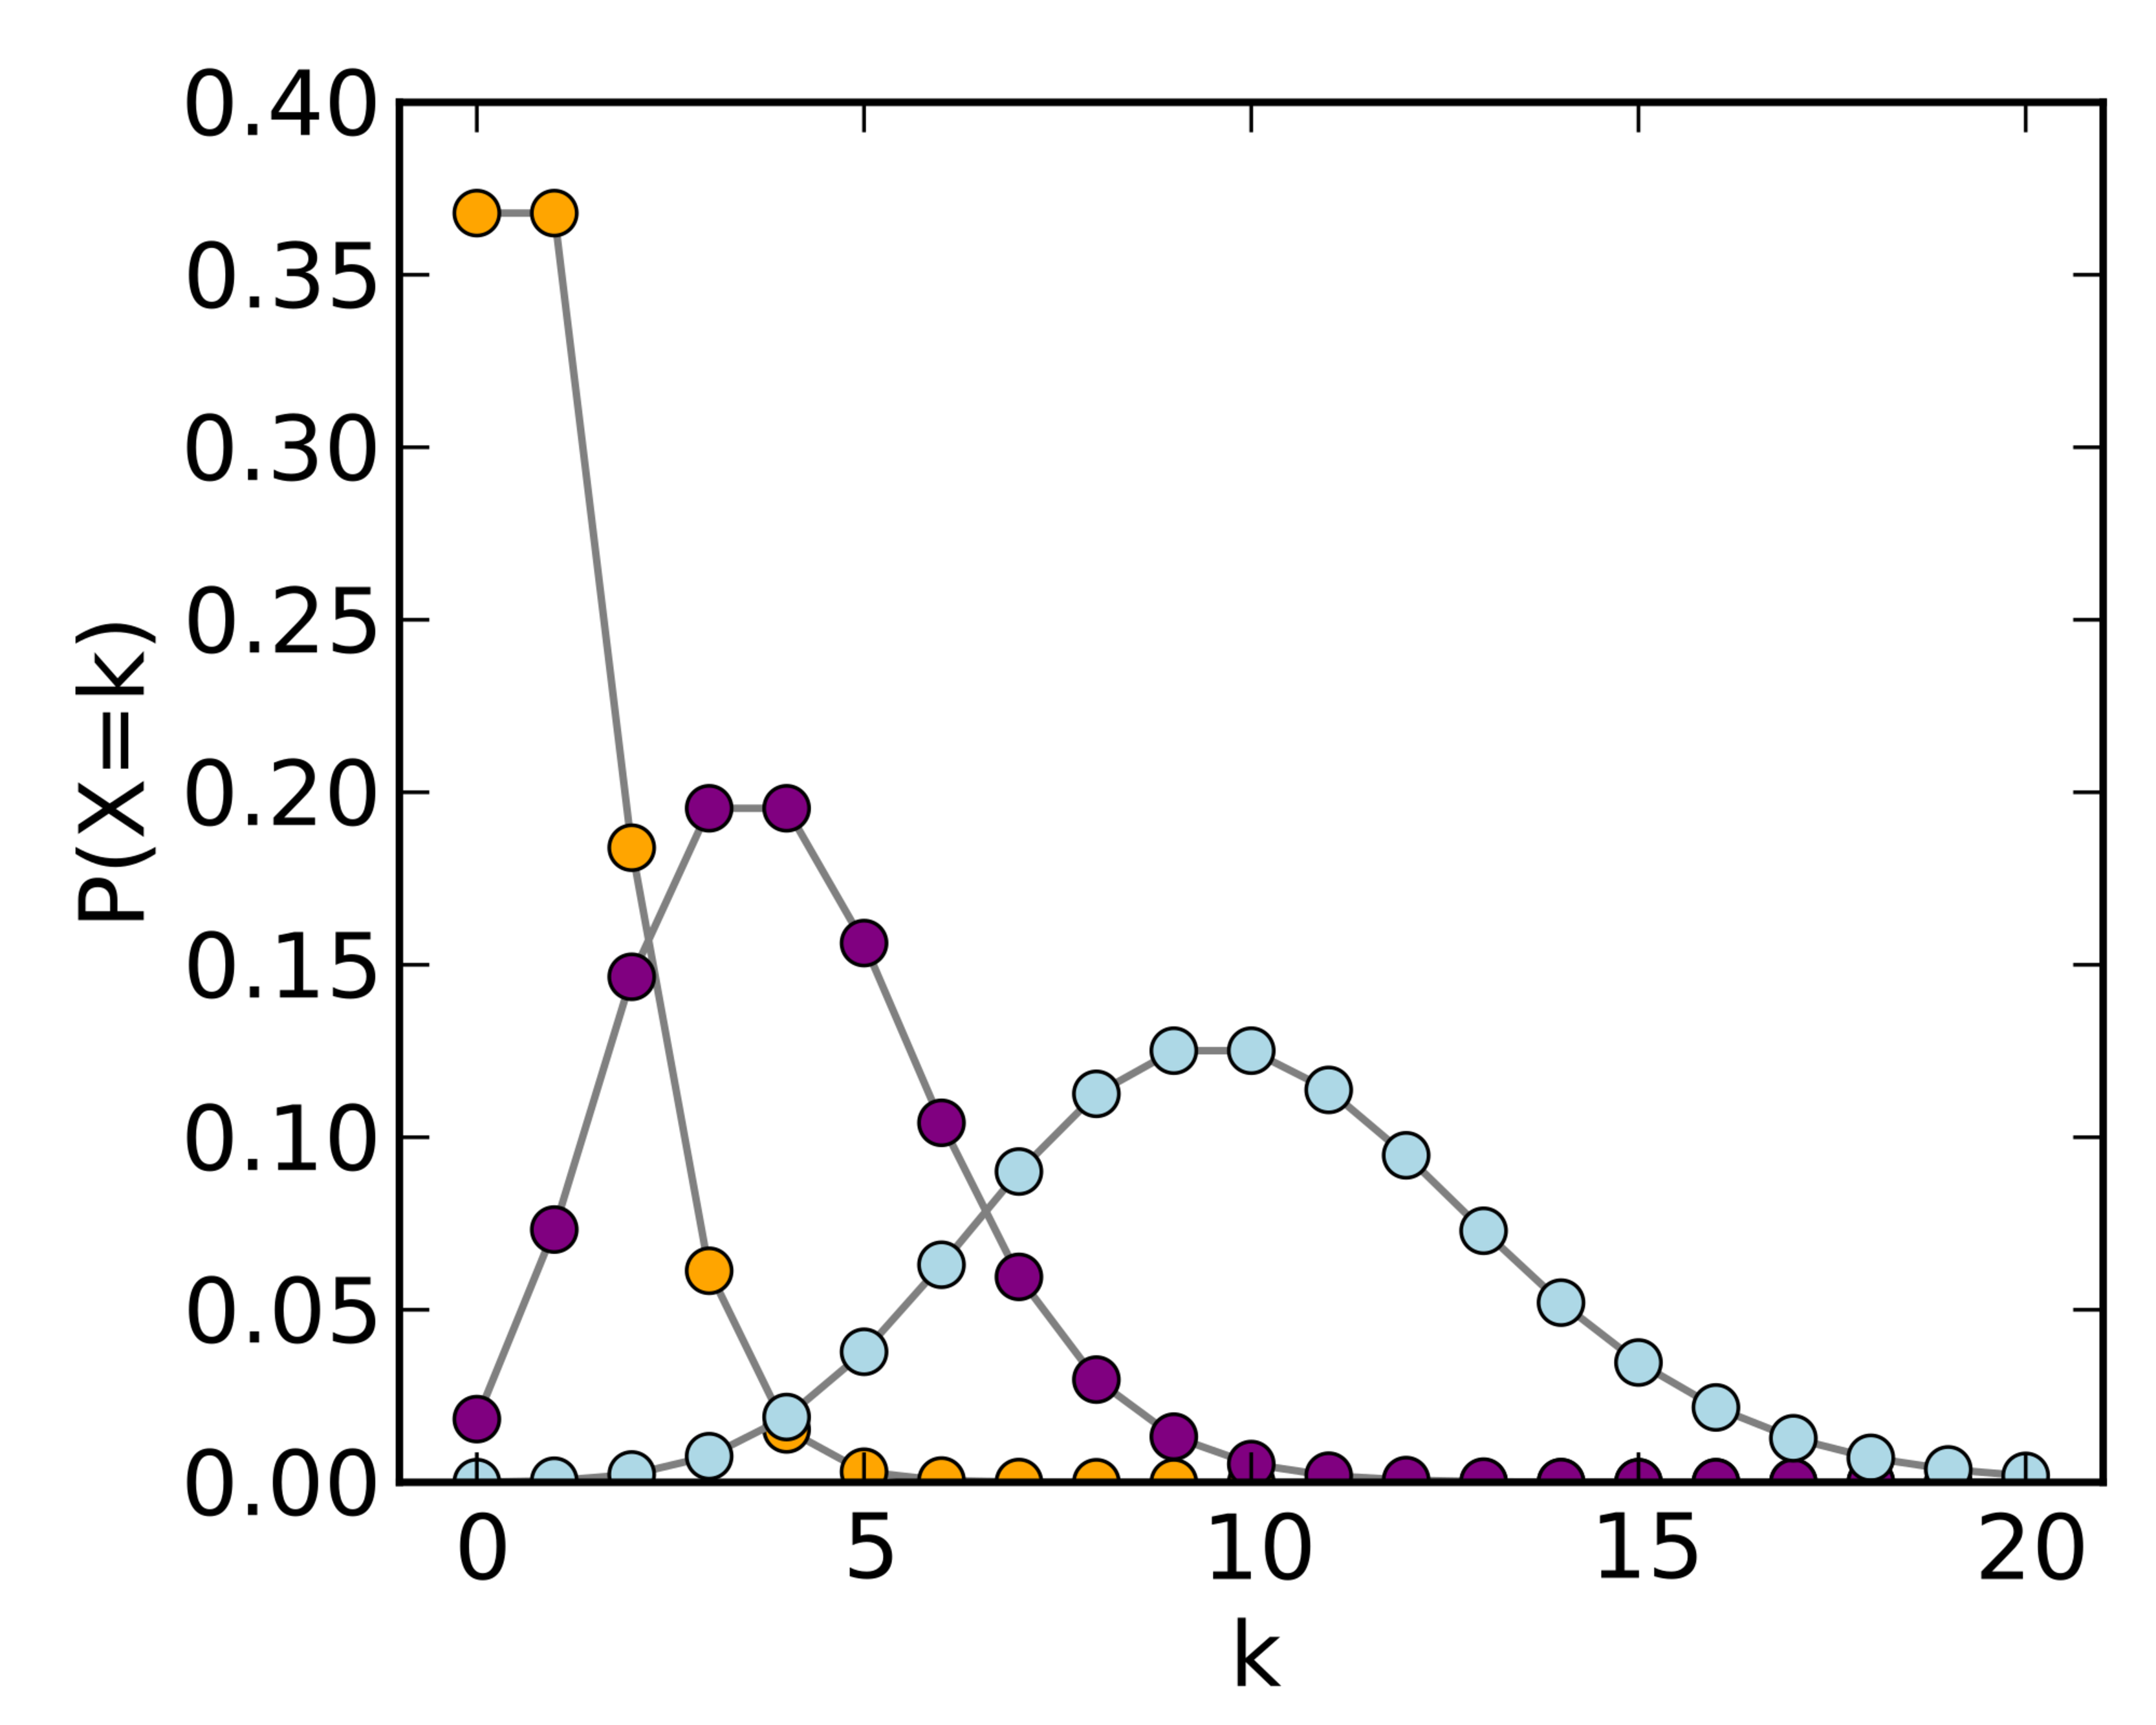
\includegraphics[width = 3.3cm]{img/Binomial_pmf.pdf}}
	\parbox{3.3cm}{\emph{KVF/CDF:} \\ 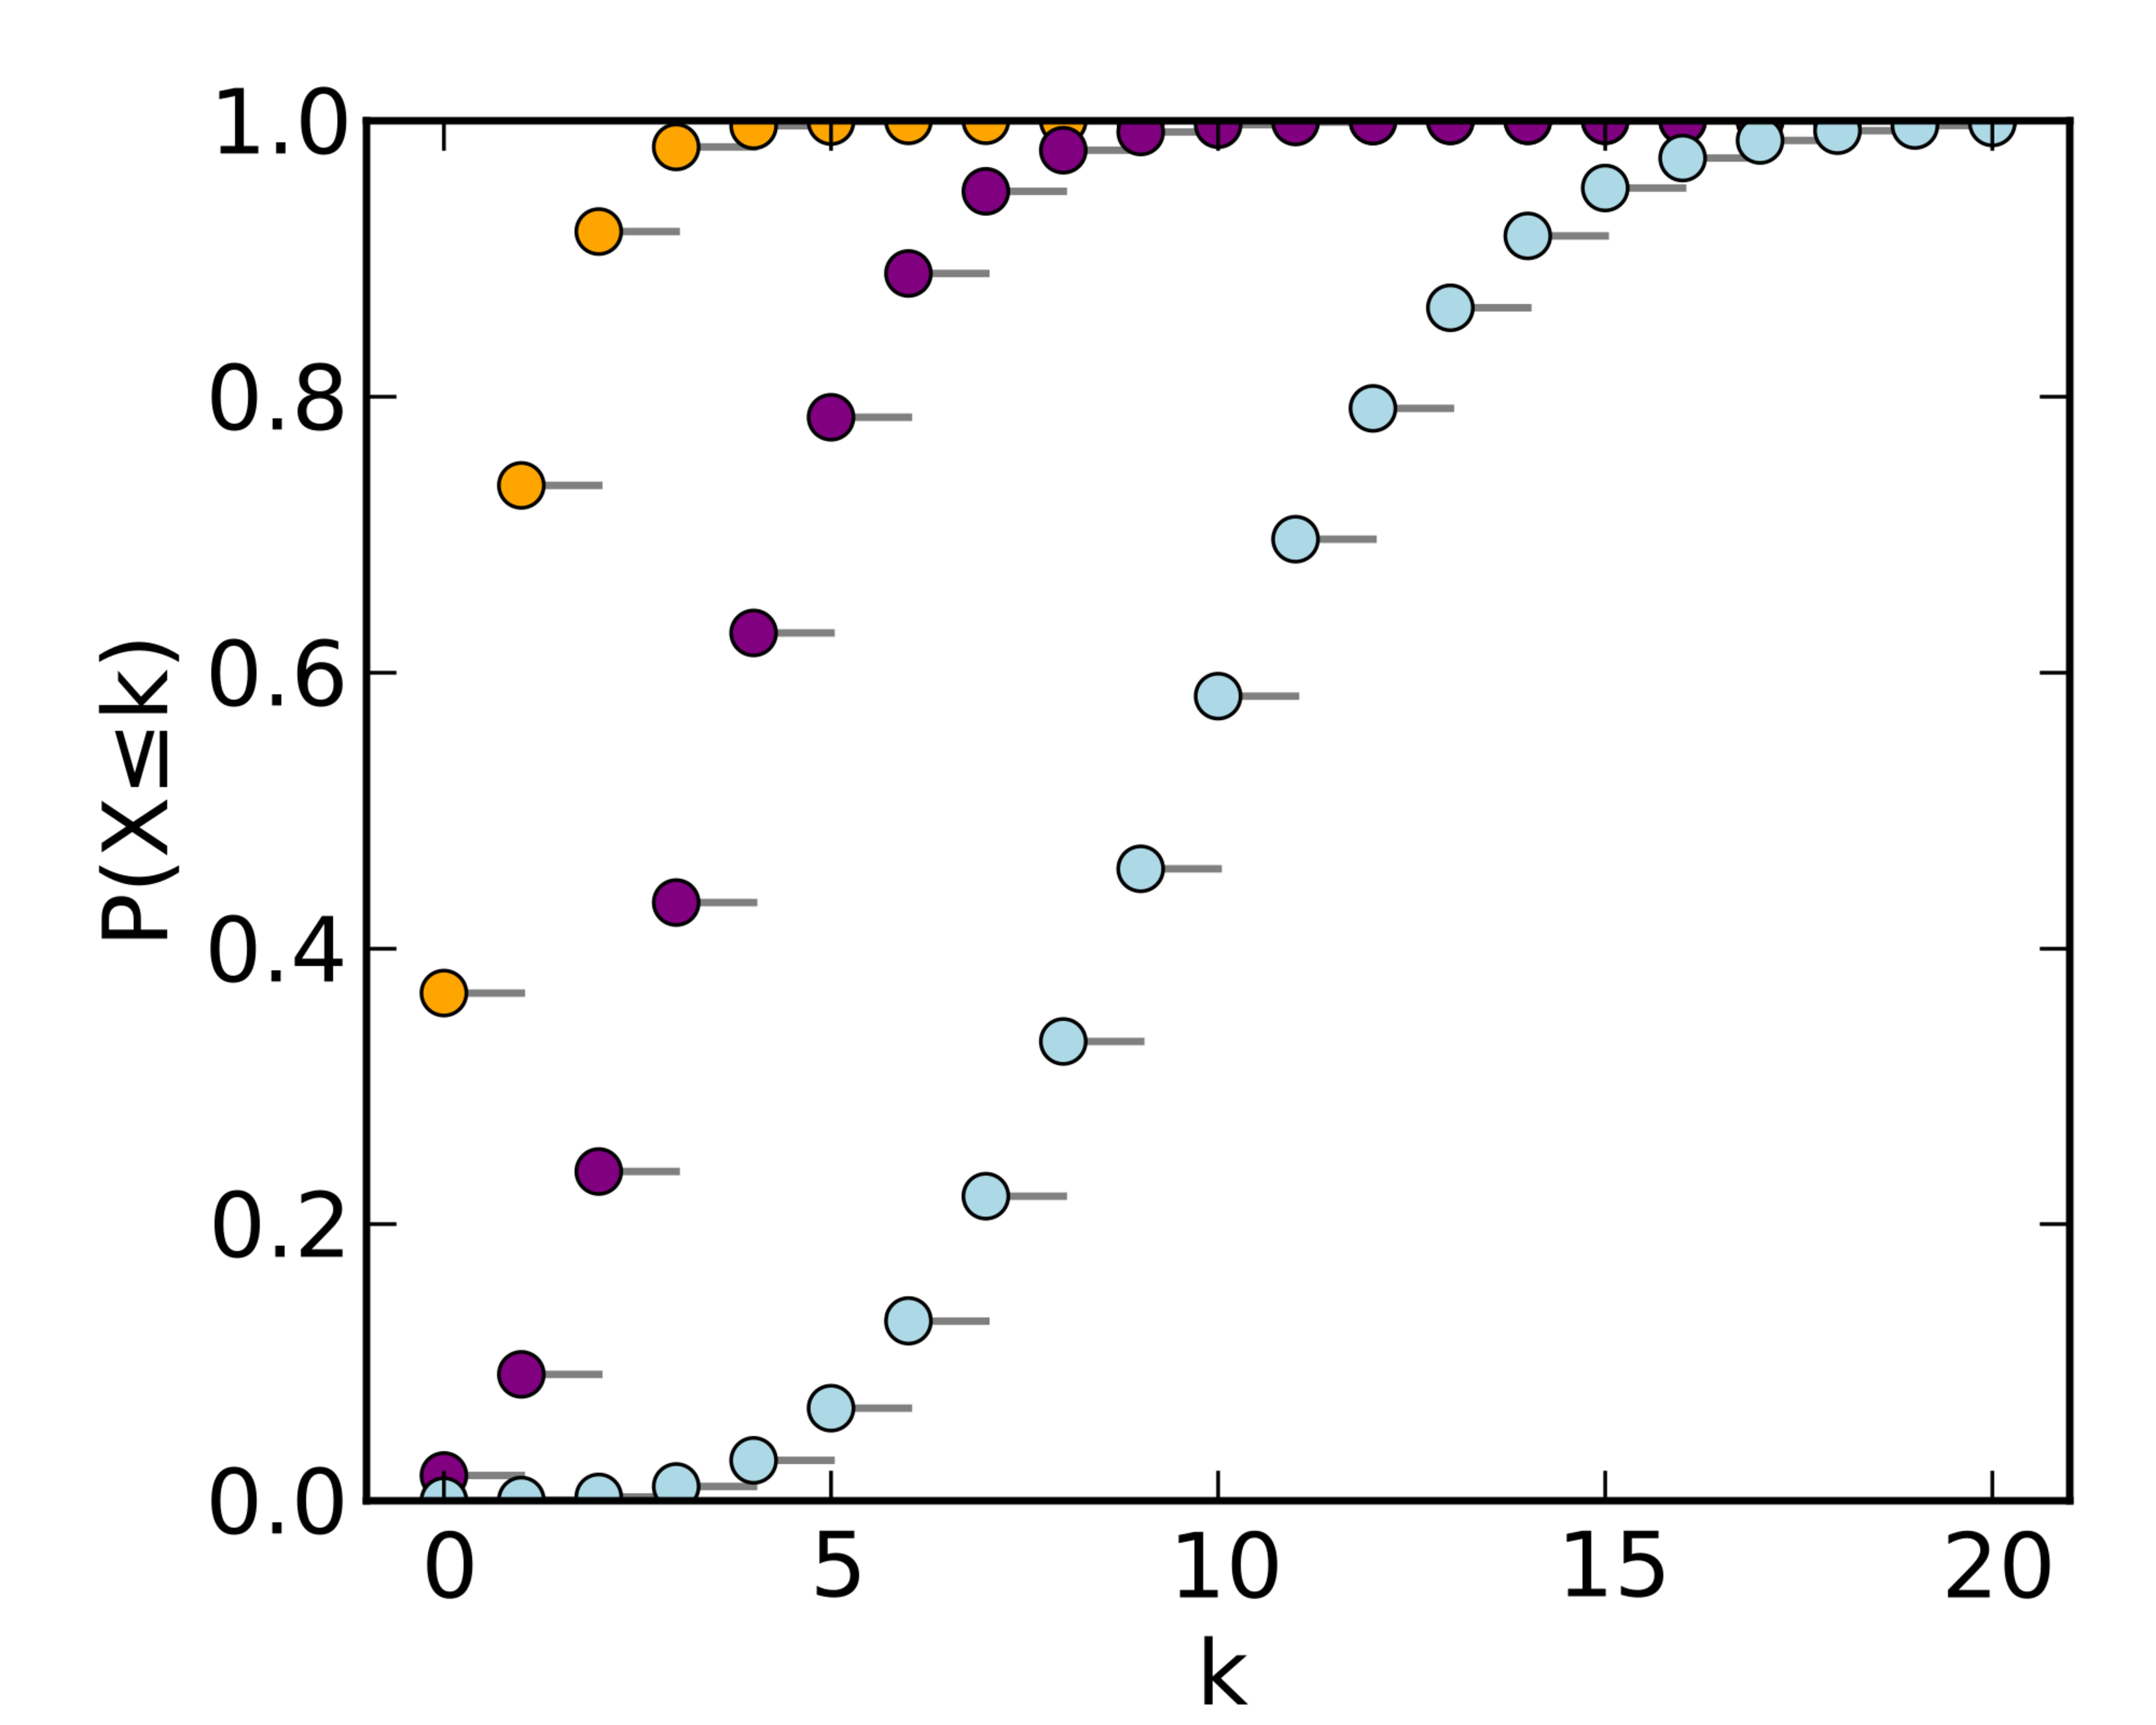
\includegraphics[width = 3.3cm]{img/Binomial_cdf.pdf}}\\
	\begin{tablebox}{l@{\extracolsep\fill}ll}
		$\underset{\text{Erwartungswert}}{\E[\X] =n p}\quad $ & $\underset{\text{Varianz}}{\Var[\X] =np (1-p)}$ & $\underset{\text{Wahrscheinlichkeitserz. Funktion}}{G_X (z) = (pz + 1 -p)^n}$\\
	\end{tablebox}

	\emph{Charakteristische Funktion}
	\qquad$\varphi_{\X}(\cx s) = \big(1-p+pe^{\cx s}\big)^n$\\
	\emph{Beispiele:} Anzahl der Übertragungsfehler in einem Datenblock endlicher Länge, Wiederholtes Werfen einer Münze
\end{sectionbox}

% ====================================================================================
\begin{sectionbox}
	\subsection{Poisson-Verteilung ($\lambda \ge 0$)}
	Asymptotischer Grenzfall der Binomialverteilung\\
	$n \ra \infty, p \ra 0, np \ra \lambda$ \quad $p_{\X}(k) = \lim\limits_{n \ra \infty}{B_{n,\frac{\lambda}{n}}(k)}$\\[0.5em]
	\parbox{3.3cm}{\emph{WMF/PMF:} \\ $p_{\X}[k] = \frac{\lambda^k}{k!} e^{-\lambda}$ \qquad $k \in \N_0$\\ 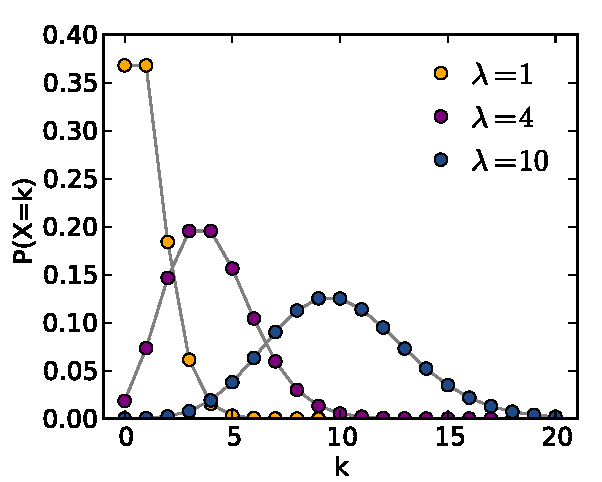
\includegraphics[width = 3.3cm]{img/poisson_pmf.pdf}}
	\parbox{3.3cm}{\emph{KVF/CDF:} \\ $F_{\X}[k] =$ zu kompliziert \\ 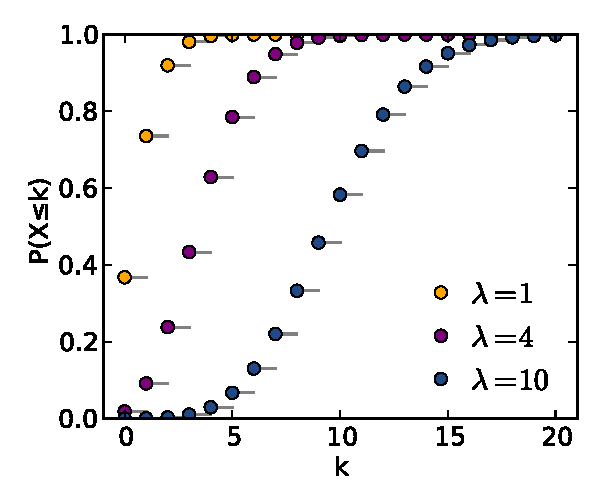
\includegraphics[width = 3.3cm]{img/poisson_cdf.pdf}}\\

	\everymath{\displaystyle}
	\begin{tablebox}{l@{\extracolsep\fill}ll}
		$\underset{\text{Erwartungswert}}{\E[\X] =\lambda}\quad$ & $\underset{\text{Varianz}}{\Var[\X] =\lambda}$ & $\underset{\text{Wahrscheinlichkeitserz. Funktion}}{G_X (z) = e^{\lambda(z-1)}}$\\
	\end{tablebox} \everymath{\textstyle}
	\emph{Charakteristische Funktion}
	\qquad$\varphi_{\X}(\cx s)=\exp\big(\lambda(e^{\cx s} -1)\big)$\\
	\emph{Beispiele:} Zahl der Phänomene in einem Zeitintervall, Google-Anfragen in einer Stunde, Schadensmeldungen an Versicherungen in einem Monat
\end{sectionbox}

% ====================================================================================
\begin{sectionbox}
	\subsection{Geometrische Verteilung ($p \in [0,1]$)}
	Erster Erfolg eines Bernoulli-Experiments beim $k$-ten Versuch, \emph{Gedächtnislos}\\[0.5em]
	\parbox{3.3cm}{\emph{WMF/PMF:} \\ $p_{\X}[k] = (1 - p)^{k - 1}p$, $k \in \N$ \\ 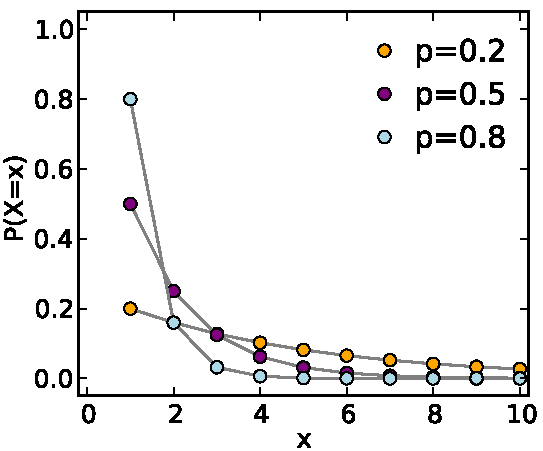
\includegraphics[width = 3.3cm]{img/geometric_pmf.pdf}}
	\parbox{3.3cm}{\emph{KVF/CDF:} \\ $F_{\X}[k] = 1-(1 - p)^k$, $k \in \N$ \\ 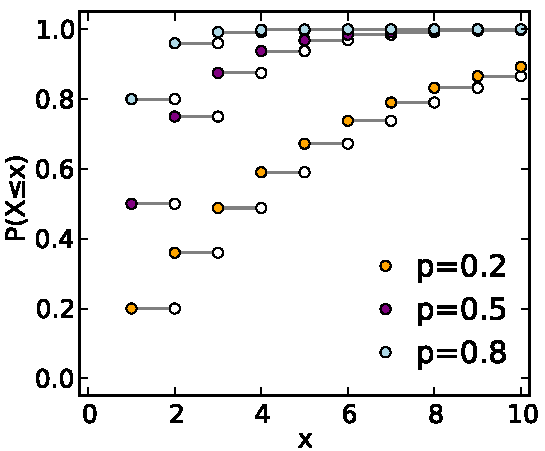
\includegraphics[width = 3.3cm]{img/geometric_cdf.pdf}}\\


	\everymath{\displaystyle}
	\begin{tablebox}{l@{\extracolsep\fill}ll}
		$\underset{\text{Erwartungswert}}{\E[\X] =\frac{1}{p}}$ & $\underset{\text{Varianz}}{\Var[\X] =\frac{1-p}{p^2}}$ & $\underset{\text{Wahrscheinlichkeitserz. Funktion}}{G_X (z) = \frac{pz}{1-z+pz}}$\\
	\end{tablebox}
	\emph{Charakteristische Funktion}
	\qquad $\varphi_{\X}(\cx s) = \frac{p e^{\i \cx s}}{1-(1-p)e^{\i \cx s}}$\\
	\emph{Beispiele:} diskrete Dauer bis ein technisches Gerät zum ersten Mal ausfällt, Anzahl der Würfe bis man eine "6" würfelt
\end{sectionbox}

% ====================================================================================
\begin{sectionbox}
	\subsection{Exponentialverteilung ($\lambda > 0$)}
	Wie geometrische Verteilung für stetige Zufallsvariablen ("'Lebensdauer"'), \emph{Gedächtnislos}\\
	= Wartezeit bis zum ersten Auftreten eines Ereignisses\\[0.5em]
	\parbox{3.3cm}{\emph{WDF/PDF:}\\ $f_{\X}(x) = \lambda e^{-\lambda x}$ \qquad$x \geq 0$\\ 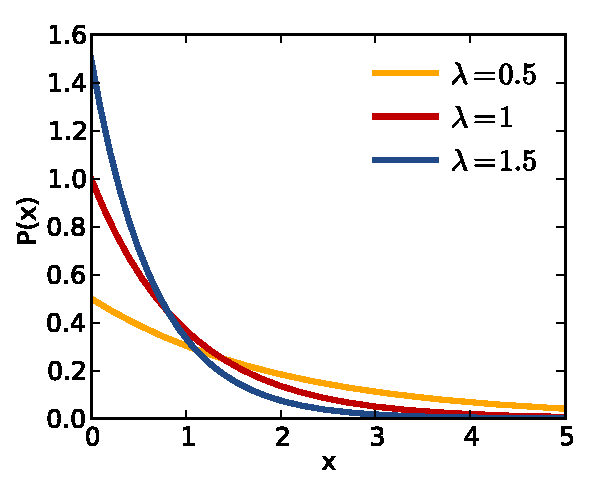
\includegraphics[width = 3.3cm]{img/exponential_pdf.pdf}}
	\parbox{3.3cm}{\emph{KVF/CDF:} \\ $F_{\X}(x) = 1-e^{-\lambda x}$ \qquad$x \geq 0$ \\ 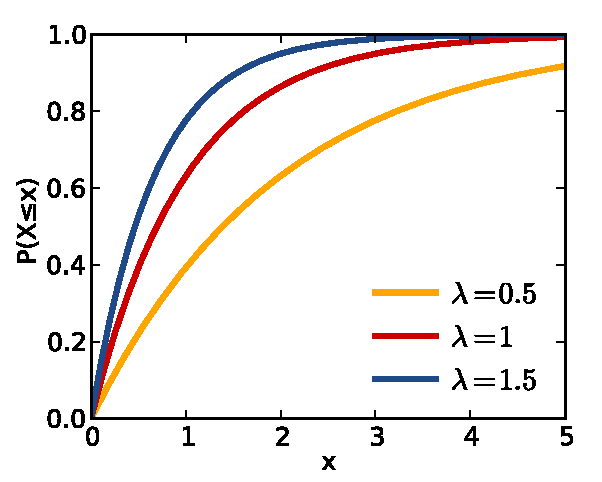
\includegraphics[width = 3.3cm]{img/exponential_cdf.pdf}}\\
	\everymath{\displaystyle}
	\begin{tablebox}{l@{\extracolsep\fill}ll}
		$\underset{\text{Erwartungswert}}{\E(\X) =\frac{1}{\lambda}}$ & $\underset{\text{Varianz}}{\Var(\X) =\frac{1}{\lambda^2}}$ & $\underset{\text{Charakt. Funktion}}{\varphi_{\X}(\omega) = \frac{\lambda}{\lambda-j\omega}}$\\
	\end{tablebox}
	\emph{Beispiele:} Lebensdauer von el. Bauteilen, Zeitdauer zwischen zwei Anrufen in einem Call-Center
\end{sectionbox}

\begin{sectionbox}
	\subsection{Normalverteilung ($\mu \in \R , \sigma > 0$)}
	\parbox{3.3cm}{\emph{WDF/PDF:} \\ 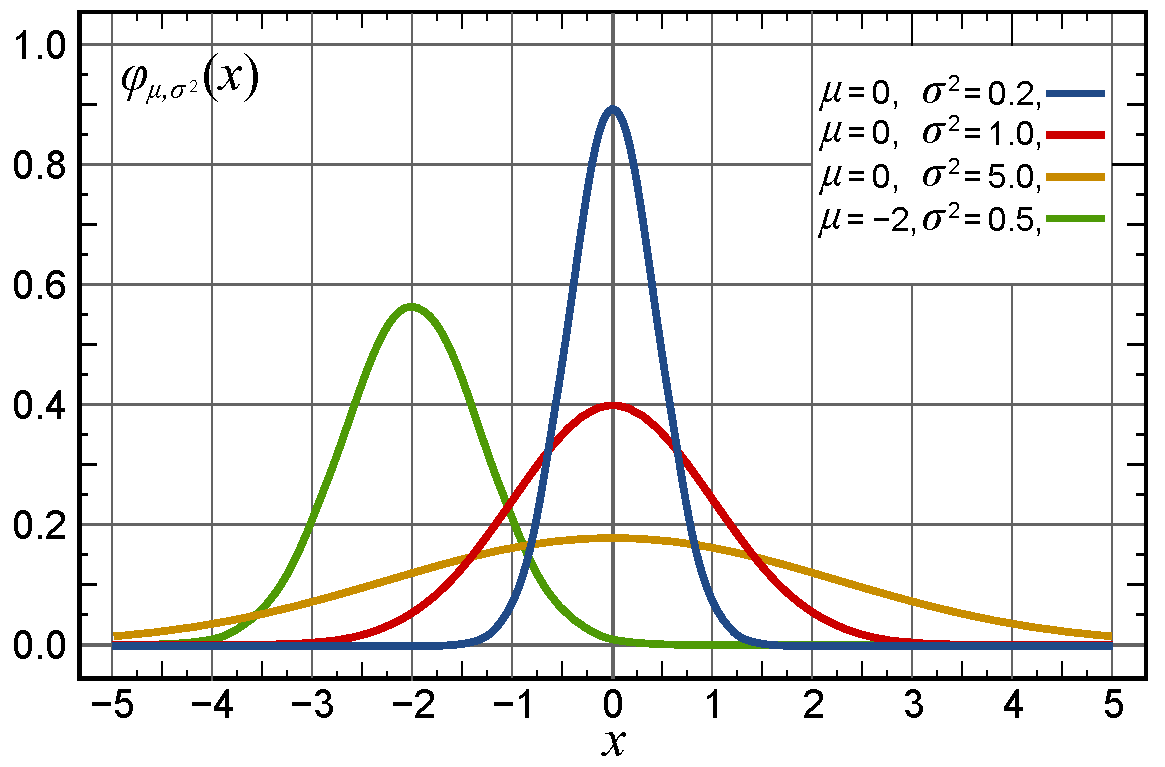
\includegraphics[width = 3.3cm]{img/normal_pdf.pdf}}
	\parbox{3.3cm}{\emph{KVF/CDF:} \\ 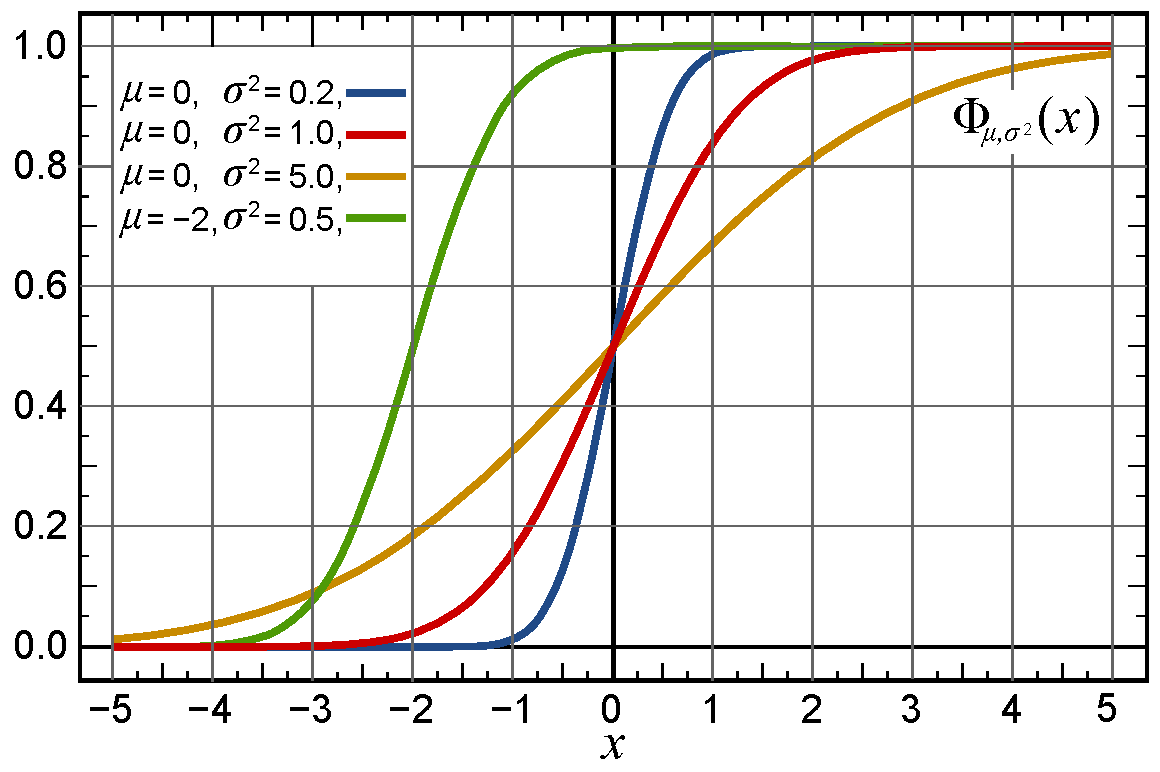
\includegraphics[width = 3.3cm]{img/normal_cdf.pdf}}\\
	\paragraph{WDF}
	\boxed{f_X (x) = \frac{1}{\sqrt{2 \pi \sigma^2}} e^{-\frac{(x-\mu)^2}{2 \sigma^2}} \quad x \in \mathbb R}

	\everymath{\displaystyle}
	\begin{tablebox}{l@{\extracolsep\fill}ll}
		$\underset{\text{Erwartungswert}}{\E(\X) = \mu}$ & $\underset{\text{Varianz}}{\Var(\X) =\sigma^2}$ & $\underset{\text{Charakt. Funktion}}{\varphi_{\X}(\omega) = e^{j\omega\mu-\frac{\omega^2\sigma^2}{2}}}$\\
	\end{tablebox}
	\emph{Schreibweise} $\X \sim \mathcal{N} (\mu,\sigma^2)$ \\
	\emph{Beispiele:} Rauschen, Ort eines Teilchens relativ zu seiner Anfangsposition bei brownscher Molekularbewegung, abgefahrene Sachen, die man nicht genauer bestimmen will oder kann
	\subsubsection{Standartnormalverteilung}
	ist der Spezialfall $\X \sim \mathcal{N} (0,1)$\\
	$\phi(x) = \frac{1}{\sqrt{2\pi}}e^{{-\frac{x^2}{2}}}$\\
	Es gilt außerdem:
	\begin{itemize}
		\item $\Y \sim \mathcal{N}(\mu,\sigma^2) \Ra \X = \frac{1}{\sigma}(\Y - \mu) \sim \mathcal{N}(0,1)$
		\item $\X \sim \mathcal{N}(0,1) \Ra \Y = \sigma \X + \mu \sim \mathcal{N}(\mu,\sigma^2)$
	\end{itemize}
\end{sectionbox}

% ----------------------------------------------------------------------------
% | Erwartungswert und Varianz |
% ~~~~~~~~~~~~~~~~~~~~~~~~~~~~~~~~~~~~~~~~~~~~~~~~~~~~~~~~~~~~~~~~~~~~~~~~~
% SECTION ====================================================================================
\section{Erwartungswert}
% ============================================================================================
\begin{sectionbox}
	\subsection{Erwartungswert}
	gibt den mittleren Wert einer Zufallsvariablen an

	\begin{emphbox}
		$\E [\X] = \underset{\text{diskrete} \X:\Omega \ra \Omega'}{\sum\limits_{x \in \Omega'} x \cdot \P_{\X}(x)} \quad \stackrel{\wedge}{=}\quad \underset{\text{stetige} \X: \Omega \ra \R}{\int \limits_{\R} x \cdot f_{\X} (x) \diff x}$
	\end{emphbox}
	Eigenschaften:
	\begin{tablebox}{ll}
		Linearität: &
		$E[\alpha \X + \beta \Y] = \alpha E [\X] + \beta E[\Y]$ \\
		Monotonie: &
		$\X \le \Y \Ra E[\X] \le E[\Y]$ \\
	\end{tablebox}
	Beweis mit der Definition und der Linearität des Integrals bzw. der Summe. \\
	\\
	$\E[\X\Y] = \E[\X] \E[\Y]$, falls $\X$ und $\Y$ stochastisch unabhängig\\
	Umkehrung nicht möglich: Unkorrelliertheit $\not \Ra$ Stoch. Unabhängig! \\
	\\
	$\E[\X\Y]= \int \limits_{\R}\int \limits_{\R}  xy \cdot f_{X,Y} (x,y) \diff x \diff y$\\
	\\
	Spezialfall für $\X: \Omega \ra \mathbb R_+$: \\
	$\E[\X] = \int \limits_0^\infty \P(\X > t) \diff t$ (stetig) \qquad $\E[\X] = \sum \limits_{k=0}^{\infty} \P(\X >k)$ (diskret)

	\subsubsection{Für Funktionen von Zufallsvariablen $g: \mathbb R \ra \mathbb R$}
	$\E[g(\X)] = \sum \limits_{x \in \Omega'} g(x) \P_{\X} (x)\quad \stackrel{\wedge}{=}\quad \int \limits_{\R} g(x) f_X (x) \diff x$
\end{sectionbox}

% SECTION ====================================================================================
\section{Varianz und Kovarianz}
% ============================================================================================
\begin{sectionbox}
\subsection{Varianz}
	ist ein Maß für die Stärke der Abweichung vom Erwartungswert
	\begin{emphbox}
		$\Var [X] = \E \big[(\X - \E[\X])^2\big] = \E[\X^2] - \E[\X]^2$
	\end{emphbox}
	$\Var [ \alpha \X + \beta] = \alpha^2 \Var [\X]$ \hfill $\Var [\X] = \Cov [\X,\X]$\\[0.5em]
	$\Var \left[\sum \limits_{i=1}^n \X_i \right] = \sum \limits_{i=1}^{n} \Var [\X_i] + \sum\limits_{j \not= i} \Cov[\X_i, \X_j]$
	\subsubsection{Standard Abweichung}
	$\sigma = \sqrt{\Var[\X]}$
\end{sectionbox}

% SECTION ====================================================================================
\section{Erzeugende und charakter. Funktionen}
% ============================================================================================

\begin{sectionbox}
	\subsection{Wahrscheinlichkeitserzeugende Funktion}
	für $\X : \Omega \ra \mathbb N_0$

	\boxed{G_{\X} (z) = \E[z^{\X}] = \sum \limits_{k=0}^\infty p_{\X} (k) z^k, \quad \abs{z} \le 1}

	\paragraph{Anwendungen}
	\begin{eqnarray*}
		p_{\X}(n) =\P(\eset{\X = n}) = \frac{1}{n!} [\frac{\diff^n}{\diff z^n} G_{\X} (z)]_{z = 0}, \quad \forall n \in \mathbb N_0 \\
		\E [\X] = [\frac{\diff}{\diff z} G_{\X} (z)]_{z = 1} \\
		\E [\X^2]-\E[\X] = [\frac{\diff^2}{\diff z^2} G_{\X} (z)]_{z = 1} \\
		\Var [\X] =[\frac{\diff^2}{\diff z^2} G_{\X} (z)]_{z = 1} - \E [\X]^2 + \E [\X]
	\end{eqnarray*}
	Für $\X_i : \Omega \ra \mathbb N_0, i \in \eset{1, \ldots, n}$ stochastisch unabhängige, diskrete, nichtnegative ZV und $\Z = \sum_{i=1}^{n} \X_i$
	\[G_{\Z} (z) = \prod_{i = 1}^{n} G_{\X_i} (z)\]

\end{sectionbox}

% Im WS2015/16 nicht Klausurrelevant
%\begin{sectionbox}
%	\subsection{Momenterzeugende Funktion} % (fold)
%	\label{sub:momenterzeugende_funktion}
%
%	Mit $\X: \Omega \ra \mathbb R$ eine reelle ZV: \\
%
%	\boxed{
%		M_{\X} (s) = \E [e^{s \X}], \quad s \in \mathbb D = \eset{s \in \mathbb R }{\E [e^{s \X} < \infty]}
%	}\\
%
%
%	Potenzreihenentwicklung (mit $s \in ]-a, a[$):\\
%	$M_{\X} (s) = \E [ e^{s \X}] = \E \left[\sum \limits_{k=0}^{\infty} \frac{s^k}{k!} \X^k\right] = \sum \limits_{k=0}^{\infty} \frac{s^k}{k!} \E\left[\X^k\right]$
%
%	Erwartungswert:
%	$\E[\X^n] = \left[\frac{\diff^n}{\diff s^n} M_{\X} (s)\right]_{s=0}, \quad \forall n \in \mathbb N_0$
%
%	Summe von ZV:
%	$M_{\Z} (s) = \prod \limits_{i = 1}^{n} M_{\X_i} (s)$
%\end{sectionbox}

% subsection momenterzeugende_funktion (end)
\begin{sectionbox}
	\subsection{Charakteristische Funktion} % (fold)
	\label{sub:charakteristische_funktion}
	\boxed{\varphi_{\X} (\omega) = \ew{e^{\i \omega \X}} , \quad \omega \in \mathbb R} $\qquad \varphi_{\X} = \int\limits_{-\infty}^\infty e^{\i\omega x} f_{\X}(x) \diff x$\\
	$f_{\X}(-x) \T \varphi(\omega)$ \\

	\emph{Erwartungswert:}
	\begin{eqnarray*}
		\E[\X^n] = \frac{1}{\i^n} \left[\frac{\diff^n}{\diff \omega^n} \varphi_{\X}(\omega)\right]_{\omega = 0}
	\end{eqnarray*}
	\emph{Summe von ZV:} $Z=\sum_{i=1}^{n}X_i$
	\begin{eqnarray*}
		\varphi_{\Z} (\omega) = \prod_{i=1}^{n} \varphi_{\X_i} (\omega)
	\end{eqnarray*}
\end{sectionbox}

% subsection charakteristische_funktion (end)
\begin{sectionbox}
	\subsection{Der zentrale Grenzwertsatz}
	\emph{Definition}: Seien $\X_i, i \in {1,...,n}$, stochastisch unabhängige und identisch
	verteilte reelle Zufallsvariablen und gelte $E[\X_i] = \mu < \infty$ und $Var[\X_i] = \sigma^2 < \infty$.
	Dann konvergiert die Verteilung der standardisierten Summe\\
	\centerline{$\Z_n= \sum\limits_{i=1}^{n}\frac{(\X-\mu)}{\sigma\sqrt{n}}$} \\
	d.h $E[\Z_n] = 0$ und $Var[\Z_n] = 1$, für $n \ra \infty$ gegen die Standartnormalverteilung. \\
	Es gilt also: \\
	\centerline{$\lim_{n \ra \infty} \P({\Z_n \le z}) = \Phi (z)$}
\end{sectionbox}
% subsection der_zentrale_grenzwertsatz (end)


\vfill
%\columnbreak

% SECTION ====================================================================================
\section{Reelle Zufallsfolgen}
% ============================================================================================

\begin{sectionbox}
	\subsection{Markow-Ungleichung}
	\boxed{\P(\eset{\abs{\X} \ge a}) \le \frac{\E[|\X|]}{a} }
\end{sectionbox}

\begin{sectionbox}
	\subsection{Tschebyschow-Ungleichung}
	\boxed{\P(\eset{\abs{\X- \E[\X]} \ge a}) \le \frac{\Var[\X]}{a^2} }


\end{sectionbox}
\begin{sectionbox}
	\subsection{Das schwache Gesetz der großen Zahlen}
	Sei $(\X_i : i \in \N)$ eine Folge reeller, paarweise unkorrelierter Zufallsvariablen mit beschränkter Varianz:\\
	$\frac{1}{n} \sum\limits_{i = 1}^n (\X_i - \E[\X_i]) \ra 0$\\ \\
	Für stochastisch unabhängige und identisch verteilte Folgenelemente mit $E[\X_i] = E[X]$ und $Var[\X_i] = Var[X] < \infty$ gilt: \\
	$\frac{1}{n} \sum\limits_{i = 1}^n (\X_i) \ra \E[\X_i] $
\end{sectionbox}

% SECTION ====================================================================================
\section{Markowketten}
\begin{sectionbox}
	\subsection{Markowketten}
	\subsubsection{Allgemein}
	Eine Zufallsfolge ($\mathsf{\X}_{n}: n \in \mathbb{N}$) heißt Markowkette, falls $\forall \ n_{i} \in \N, \\
	i \in {1, \dots k}$ mit $n_{1} < \dots < n_{k}$ gilt:\\
	$\mathsf{(\X_{n_{1}},\X_{n_{2}}, \dots \X_{n_{k-2}}) \ra \X_{n_{k-1}} \ra \X_{n_{k}}}$ \\
	$\Ra$ Die Verteilung eines Folgeelements hängt nur vom direkten Vorgänger ab
	\begin{tablebox}{@{\extracolsep\fill}l@{}}
	$p_{\X_{n_k}|\X_{n_{k-1}},\X_{n_{k-2}},...,\X_{n_1}}(x_{n_k}|x_{n_{k-1}},x_{n_{k-2}},...,x_{n_1})$ \\
	$=p_{\X_{n_k}|\X_{n_{k-1}}}(x_{n_k}|x_{n_{k-1}})$ \\
	\end{tablebox}

	\begin{tablebox}{@{\extracolsep\fill}l@{}}
	$f_{\X_{n_k}|\X_{n_{k-1}},\X_{n_{k-2}},...,\X_{n_1}}(x_{n_k}|x_{n_{k-1}},x_{n_{k-2}},...,x_{n_1})$ \\
	$=f_{\X_{n_k}|\X_{n_{k-1}}}(x_{n_k}|x_{n_{k-1}})$
	\end{tablebox}

	\subsubsection{Zustandsübergang}
	\emph{Zustandsübergangswahrscheinlichkeit:} \\
	\centerline{$p_{\X_{n} | \X_{n-1}}(x_{n} | x_{n-1})$}\\

	\qquad Verbund-WMF: \\
	$p_{\X_1,...,\X_n}(x_1,...,x_n)=p_{\X_1}(x_1)\prod\limits_{i=2}^{n}p_{\X_i|\X_{i-1}}(x_i|x_{i-1})$ \\

	\emph{Zustandsübergangsdicht:} \\
	\centerline{$ f_{\X_{n} | \X_{n-1}}(x_{n} | x_{n-1})$}\\

	\qquad Verbund-WDF: \\
	$f_{\X_1,...,\X_n}(x_1,...,x_n)=f_{\X_1}(x_1)\prod\limits_{i=2}^{n}f_{\X_i|\X_{i-1}}(x_i|x_{i-1})$ \\ \\


	Eine Markowkette heißt \emph{homogen}, wenn die Übergangswahrscheinlichkeit\ unabhängig vom Index ist \\
	$p_{\X_{n+1} | \X_{n}} (x_{n+1} | x_{n}) = p_{\X_{n+1+k} | \X_{n+k}} (x_{n+1} | x_{n})$ \\
	$f_{\X_{n+1} | \X_{n}} (x_{n+1} | x_{n}) = f_{\X_{n+1+k} | \X_{n+k}} (x_{n+1} | x_{n})$ \\


	\subsubsection{Chapman-Kologorow Gleichung}
	2-Schritt-Übergangswahrscheinlichkeit: \\
	 $p_{\X_{n+2}|\X_n}(x_{n+2}|x_n)= \\ \sum\limits_{\xi\in\mathbb{X}}p_{\X_{n+2}|\X_{n+1}}(x_{n+2}|\xi)p_{\X_{n+1}|\X_n}(\xi |x_n)$

	m+l-Schritt-Übergangswahrscheinlichkeit: \\
	$p_{\X_{n+m+l}|\X_n}(x_{n+m+l}|x_n) =$\\
	\resizebox{\textwidth}{!}{$ \sum\limits_{\xi \in \mathbb{X}}p_{\X_{n+m+l}|\X_{n+m}}(x_{n+m+l}|x_{n+m})p_{\X_{n+m}|\X_{n}}(x_{n+m}|x_{n})$}
\end{sectionbox}
\begin{sectionbox}
	\subsubsection{Markowketten im endlichen Zustandsraum}
	$\vec{p}_{n} \triangleq \begin{bmatrix} p_{\X_{n}}(x_{1}) \\ p_{\X_{n}}(x_{2}) \\ \vdots \\ p_{\X_{n}}(x_{N}) \end{bmatrix} \quad \in [0,1]^{N}\text{ mit }[\vec{p}_{n}]_{i} = p_{\X_{n}}(x_{i})$ \\
	\emph{Übergangsmatrix:}
	 $\Pi = \begin{bmatrix} p_{11} & \cdots & p_{1N} \\ \vdots & \ddots &   \\ p_{N1} & & p_{NN} \end{bmatrix} \quad \in [0,1]^{N \times N}$\\

	 \emph{Übergangswahrscheinlichkeit:} $p_{ij} = p_{\X_{n+1}|\X_n}(\xi_i|\xi_j)$ \\
	 \centerline{Spaltensumme muss immer 1 ergeben!}\\
	 \begin{tablebox}{l}
		 $\vec{p}_{n+1}  = \Pi \vec{p}_{n} \quad n \in \N$ \\
		 $\vec{p}_{n+m}  = \Pi^{m} \vec{p}_{n} \quad n, m \in \N$
	 \end{tablebox}
	 Eine Verteilung heißt \emph{stationär}, wenn gilt:\\
	\[\vec{p}_{\infty}  = \Pi \vec{p}_{\infty} \]
\end{sectionbox}


\end{document}